\documentclass[letterpaper, 12pt]{article}
\usepackage[margin=1in]{geometry}
\usepackage{amsmath}
\usepackage{amssymb}
\usepackage{fancyhdr}
%\usepackage{hyperref}
%\usepackage{xcolor}
\setlength{\headheight}{15pt}
\usepackage{tikz}
\usetikzlibrary{positioning, calc}

\pagestyle{fancy}
\fancyhf{}

\rhead{
    Shengdong Li
    Calc 1
}
\rfoot{
    page \thepage
}

\usepackage{indentfirst}

\begin{document}
\title{Response to Swastik Sharma}
\author{by Shengdong Li}
\date{17 May 2020}
\maketitle

\section{Intro}
Hey Swas! Thanks for replying to my initial post! You made a really interesting point about the relationship between the power of $x$ in the numerator and the final resulting answer in solving the integral of $\int_{ }^{ }\frac{x^{2}}{\sqrt{4-x^{2}}}dx$. \par
From the table that you provided, it seemed to me that when the power of $x$ in the numerator was divisible by the value in the square root, the resulting answer requires trig substitution to be solved, but when the power of $x$ in the numerator wasn't, the resulting answer could be solved by $u$-sub. \par
This makes a lot of sense, as the non-divisible portion is then resolved when solving for the $du$ in $u$-sub. \par
I'll take you up on your offer to test this hypothesis on the next power, of $\int_{ }^{ }\frac{x^{4}}{\sqrt{4-x^{2}}}dx$.
\section{Using Trig Sub}
\begin{align}
    \intertext{First notice the form of the function under the square root...}
        & \int_{ }^{ }\frac{x^{4}}{\sqrt{4-x^{2}}}dx
    \intertext{It is clear here that the form is in $a^2-x^2$, which calls for $x=a\sin x$}
    x   & =a\sin\theta                                                                                               \\
    a^2 & =4                                                                                                         \\
    a   & =2                                                                                                         \\
    x   & =2\sin\theta\\
    dx  & =2\cos\theta d\theta
    \intertext{Now plugin $x$ values}
        & =\int_{ }^{ }\frac{\left(2\sin\theta\right)^{4}2\cos\theta d\theta}{\sqrt{4-\left(2\sin\theta\right)^{2}}}
    \intertext{Simplify}
        & =\int_{ }^{ }\frac{\left(2\sin\theta\right)^{4}2\cos\theta d\theta}{\sqrt{4-4\sin^{2}\theta}}              \\
        & =\int_{ }^{ }\frac{\left(2\sin\theta\right)^{4}2\cos\theta d\theta}{\sqrt{4\left(1-\sin^{2}\theta\right)}} \\
        & =\int_{ }^{ }\frac{\left(2\sin\theta\right)^{4}2\cos\theta d\theta}{\sqrt{4\cos^{2}\theta}}                \\
        & =\int_{ }^{ }\frac{\left(2\sin\theta\right)^{4}2\cos\theta d\theta}{2\cos\theta}                           \\
        & =\int_{ }^{ }16\sin^{4}\theta d\theta                                                                      \\
        & =16\int_{ }^{ }\sin^{4}\theta d\theta
        \intertext{Recall the half-angle identity}
&\sin^{2}\theta=\frac{1-\cos\left(2\theta\right)}{2}\\
&=16\int_{ }^{ }\left(\frac{1-\cos\left(2\theta\right)}{2}\right)^{2}d\theta\\
&=16\int_{ }^{ }\frac{1-2\cos\left(2\theta\right)+\cos^{2}\left(2\theta\right)}{4}d\theta\\
&=4\int_{ }^{ }1-2\cos\left(2\theta\right)+\cos^{2}\left(2\theta\right)d\theta\\
&=4\int_{ }^{ }d\theta-8\int_{ }^{ }\cos\left(2\theta\right)d\theta+4\int_{ }^{ }\cos^{2}\left(2\theta\right)d\theta
\intertext{Integrate what we can}
&=4\theta-4\sin\left(2\theta\right)+4\int_{ }^{ }\cos^{2}\left(2\theta\right)d\theta
\intertext{Now we use another trig identity}
&\cos^{2}\theta=\frac{1+\cos\left(2\theta\right)}{2}\\
&=4\theta-4\sin\left(2\theta\right)+4\int_{ }^{ }\frac{1+\cos\left(4\theta\right)}{2}d\theta\\
&=4\theta-4\sin\left(2\theta\right)+2\int_{ }^{ }d\theta+2\int_{ }^{ }\cos\left(4\theta\right)d\theta
\intertext{Integrate}
&=4\theta-4\sin\left(2\theta\right)+2\theta+\frac{1}{2}\sin\left(4\theta\right)
\intertext{We can combine the individual $\theta$s}
&=6\theta-4\sin\left(2\theta\right)+\frac{1}{2}\sin\left(4\theta\right)
\intertext{Now let's use $\sin\left(2\theta\right)=2\sin\theta\cos\theta$ to get rid of our $\theta$ coefficients}
&=6\theta-8\sin\left(\theta\right)\cos\left(\theta\right)+\sin\left(2\theta\right)\cos\left(2\theta\right)
\intertext{And again!}
&=6\theta-8\sin\left(\theta\right)\cos\left(\theta\right)+2\sin\left(\theta\right)\cos\left(\theta\right)\cos\left(2\theta\right)
\intertext{And use another trig identity, $\cos\left(2\theta\right)=\cos^{2}\left(\theta\right)-\sin^{2}\left(\theta\right)$}
&=6\theta-8\sin\left(\theta\right)\cos\left(\theta\right)+2\sin\left(\theta\right)\cos\left(\theta\right)\left(\cos^{2}\left(\theta\right)-\sin^{2}\left(\theta\right)\right)\\
&=6\theta-8\sin\left(\theta\right)\cos\left(\theta\right)+2\sin\left(\theta\right)\cos^{3}\left(\theta\right)-2\sin^{3}\left(\theta\right)\cos\left(\theta\right)
\intertext{Now let's make a triangle so we can put $\theta$ back in terms of $x$! Recall...}
x&=2\sin\theta\\
\frac{x}{2}&=\sin\theta
\end{align}
So our triangle is 
\begin{center}
    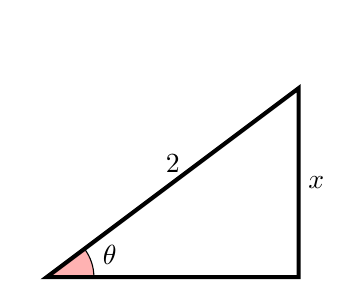
\begin{tikzpicture}[scale=0.8]
        % draw the background
        %\draw [line width=1.5pt, fill=gray!2] (0,0) -- (60:4) -- (4,0) -- cycle;

        \coordinate[label=left:$$]  (A) at (0,0);
        \coordinate[label=right:$$] (B) at (4,0);
        \coordinate[label=above:$$] (C) at (4,3);

        \coordinate[label=below:$$](c) at ($ (A)!.5!(B) $);
        \coordinate[label=above:$2$](b) at ($ (A)!.5!(C) $);
        \coordinate[label=right:$x$](a) at ($ (B)!.5!(C) $);

        %angle alpha
        \draw[fill=red!30] (0,0) -- (0:0.75cm) arc (0:36.87:.75cm);
        \draw (1cm,0.35cm) node {$\theta$};

        % angle beta
        %\begin{scope}[shift={(4cm,0cm)}]
        %    \draw[fill=green!30] (0,0) -- (-180:0.75cm) arc (180:120:0.75cm);
        %    \draw (150:0.5cm) node {$\beta$};
        %\end{scope}

        % angle gamma
        %\begin{scope}[shift={(60:4)}]
        %    \draw[fill=green!30] (0,0) -- (-120:.75cm) arc (-120:-60:.75cm);
        %    \draw (-90:0.5cm) node {$\gamma$};
        %\end{scope}

        % the triangle
        \draw [line width=1.5pt] (A) -- (B) -- (C) -- cycle;
    \end{tikzpicture}
\end{center}
Which, after solving for the third side using pythagorean theorem, gives us...
\begin{center}
    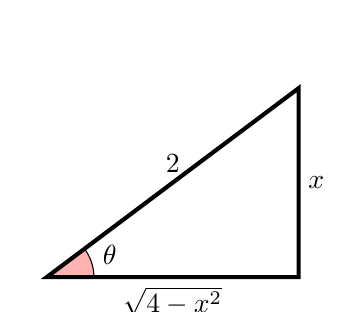
\begin{tikzpicture}[scale=0.8]
        % draw the background
        %\draw [line width=1.5pt, fill=gray!2] (0,0) -- (60:4) -- (4,0) -- cycle;

        \coordinate[label=left:$$]  (A) at (0,0);
        \coordinate[label=right:$$] (B) at (4,0);
        \coordinate[label=above:$$] (C) at (4,3);

        \coordinate[label=below:$\sqrt{4-x^2}$](c) at ($ (A)!.5!(B) $);
        \coordinate[label=above:$2$](b) at ($ (A)!.5!(C) $);
        \coordinate[label=right:$x$](a) at ($ (B)!.5!(C) $);

        %angle alpha
        \draw[fill=red!30] (0,0) -- (0:0.75cm) arc (0:36.87:.75cm);
        \draw (1cm,0.35cm) node {$\theta$};

        % angle beta
        %\begin{scope}[shift={(4cm,0cm)}]
        %    \draw[fill=green!30] (0,0) -- (-180:0.75cm) arc (180:120:0.75cm);
        %    \draw (150:0.5cm) node {$\beta$};
        %\end{scope}

        % angle gamma
        %\begin{scope}[shift={(60:4)}]
        %    \draw[fill=green!30] (0,0) -- (-120:.75cm) arc (-120:-60:.75cm);
        %    \draw (-90:0.5cm) node {$\gamma$};
        %\end{scope}

        % the triangle
        \draw [line width=1.5pt] (A) -- (B) -- (C) -- cycle;
    \end{tikzpicture}
\end{center}
\begin{align}
    \intertext{Now to solve for $\theta$ and $\cos\theta$}
    \theta&=\sin^{-1}\left(\frac{x}{2}\right)\\
    \cos\theta&=\frac{\sqrt{4-x^{2}}}{2}
    \intertext{Now we just plug everything in}
    &=6\theta-8\sin\left(\theta\right)\cos\left(\theta\right)+2\sin\left(\theta\right)\cos^{3}\left(\theta\right)-2\sin^{3}\left(\theta\right)\cos\left(\theta\right)\\
    &=6\arcsin\left(\frac{x}{2}\right)-8\left(\frac{x}{2}\right)\left(\frac{\sqrt{4-x^{2}}}{2}\right)+2\left(\frac{x}{2}\right)\left(\frac{\sqrt{4-x^{2}}}{2}\right)^{3}-2\left(\frac{x}{2}\right)^{3}\left(\frac{\sqrt{4-x^{2}}}{2}\right)
    \intertext{Now to simplify}
    &=6\arcsin\left(\frac{x}{2}\right)-2x\sqrt{4-x^{2}}+\frac{x\left(4-x^{2}\right)\sqrt{4-x^{2}}}{8}-\frac{x^{3}\sqrt{4-x^{2}}}{8}\\
    &=6\arcsin\left(\frac{x}{2}\right)+\frac{\left(x\left(4-x^{2}\right)-x^{3}-16x\right)\sqrt{4-x^{2}}}{8}\\
    &=6\arcsin\left(\frac{x}{2}\right)+\frac{\left(4x-x^{3}-x^{3}-16x\right)\sqrt{4-x^{2}}}{8}\\
    &=6\arcsin\left(\frac{x}{2}\right)+\frac{\left(-2x^{3}-12x\right)\sqrt{4-x^{2}}}{8}\\
    &=\boxed{6\arcsin\left(\frac{x}{2}\right)-\frac{\left(x^{3}+6x\right)\sqrt{4-x^{2}}}{4}+C}
\end{align}
\section{Conclusion}
So yes, it turns out that with an odd power in the numerator, you do have an $\arcsin$! Wow!\bigskip \par
Cheers, \par
Andy Li
\end{document}